
\begin{appendices}

\chapter{Peg in hole}

\section{Time to connect socket}
\label{app:anova_socket}


We aim to test if there is any significant difference in time taken to connect socket A and B. We hypothesised that socket A requires longer time than socket B. 


Data from two groups of 5 subjects where collected according the the experiment protocol.
All subjects had time to familiarise themselves with the task and accomplished multiple training rounds 
before the start of the experiment.
In Figure \ref{figuretimesubgroup} (\textit{Top row}) we plot the time taken for each subject to connect the plug 
to the socket, once the socket was localised.
 
Before applying a statistical test to compare the time taken to connect the plug to the sockets for the 
two groups, we tested the normality of the time-distribution of each experiment condition (AA, AB, BA, BB).

We applied Shapiro-Wilk test of normality in R and used Q-Q plots to compare the shapes 
of distributions (Figure \ref{QQplot}) with normality. None of the time-distributions of the experimental conditions
are normal (p< 0.0001). Therefore, we chose a non-parametric test to compare the 
distributions. Since socket A and B were performed by related samples we applied the
Wilcoxon signed-rank test (a paired difference test). This test assesses whether the population mean rank differs 
between the two sockets (A and B) given that a subject performed both experiments one after the other.

Socket A took significantly longer time than socket B and this result was observed in the two 
groups (Group A p<0.0001, Group B p=0.0002, Wilcoxon signed-rank test, Figure \ref{figuretimesubgroup}).   


\begin{figure}
 \centering
 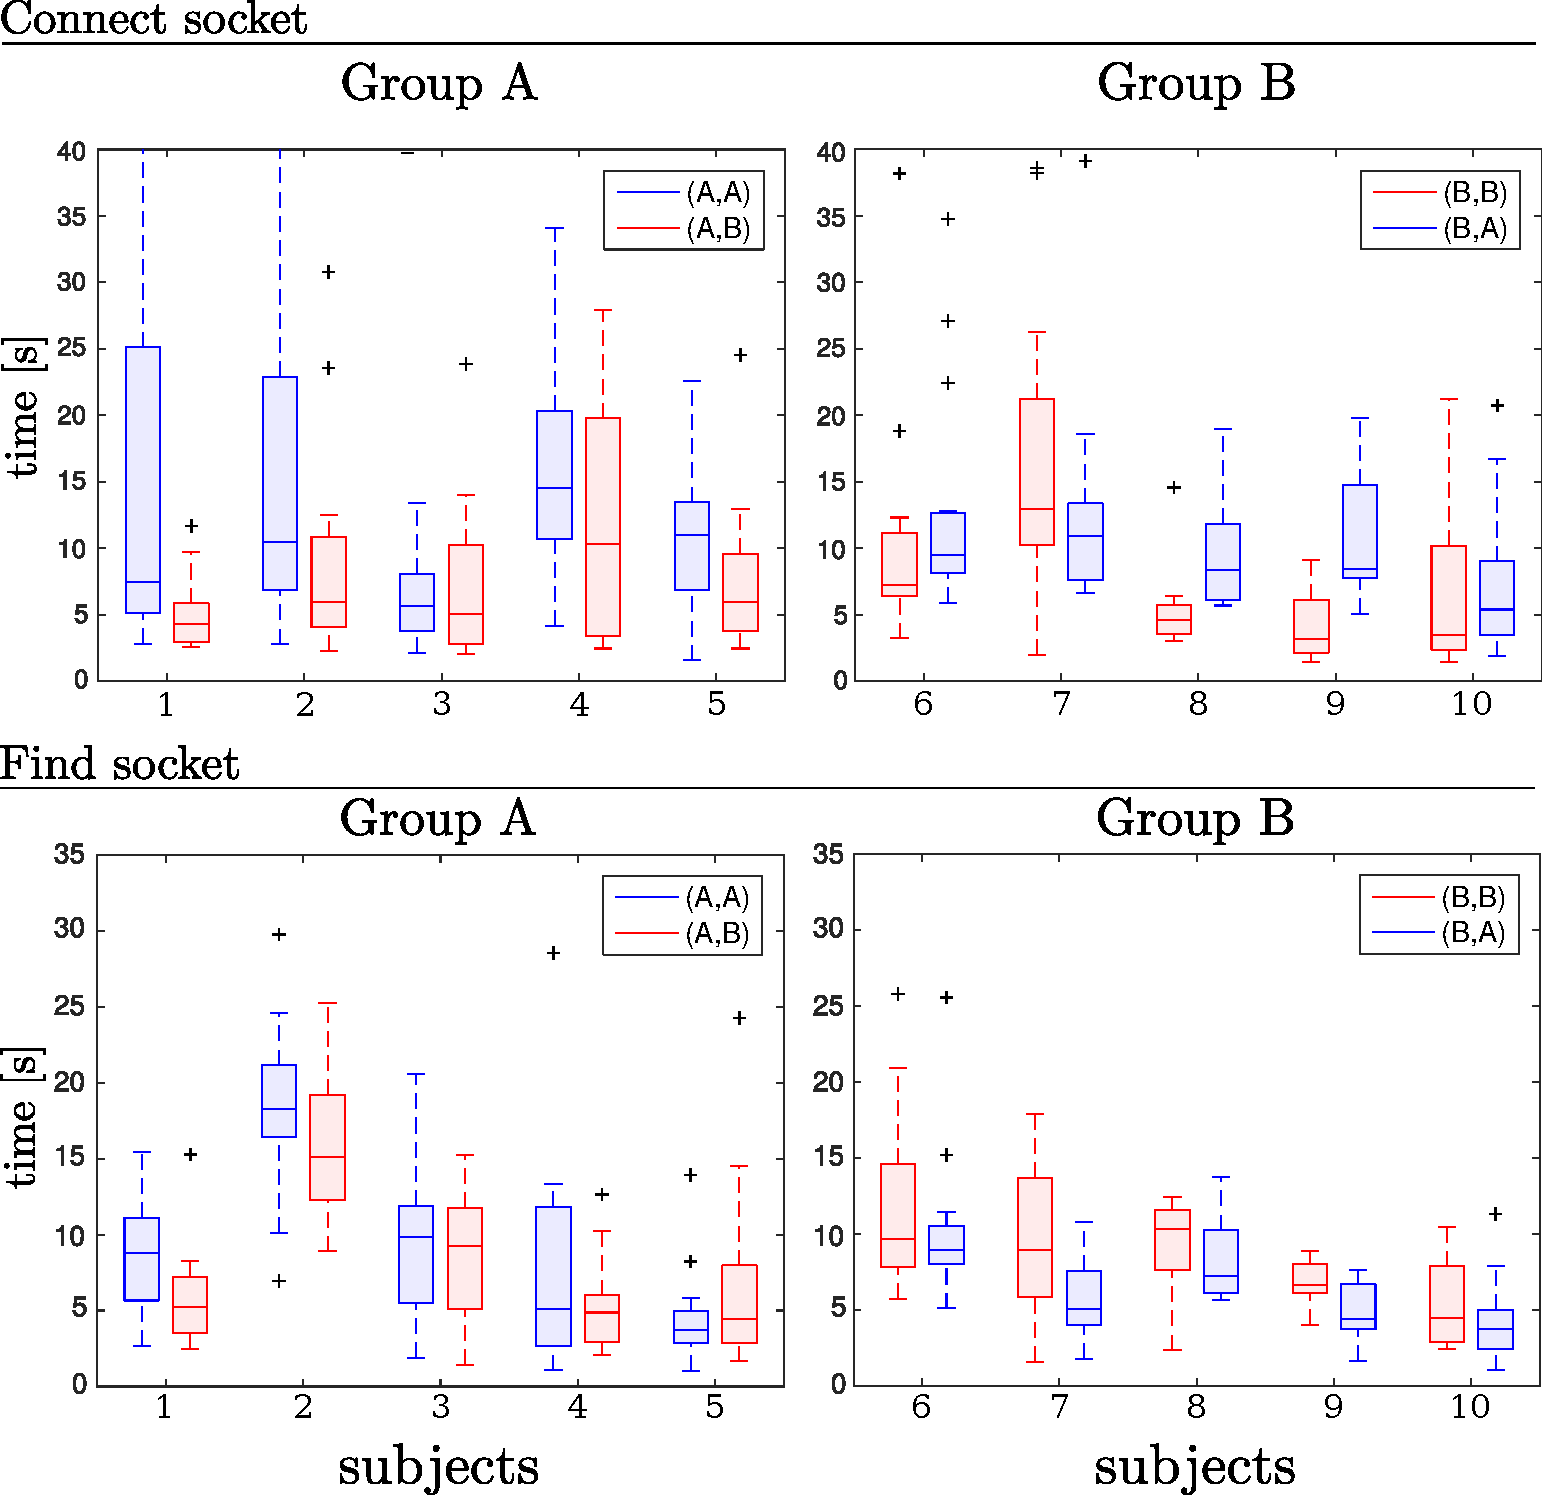
\includegraphics[width=\textwidth]{./ch4-PiH/Figures/time_taken_subgroup.pdf}
 \caption{Time taken to find and connect the plug to the power socket. \textbf{Top:} 
 Time taken to connect the plug to the socket once the socket is localised. For most subjects the median value of the taken time is higher 
 for socket A when compared with socket B. \textbf{Bottom}: time taken to localise the socket. For the second
 search, AB and BA, it seams that the subjects are faster indicating learning during the experiment.
 }
 \label{figuretimesubject}
\end{figure}

\begin{figure}	
   \centering
   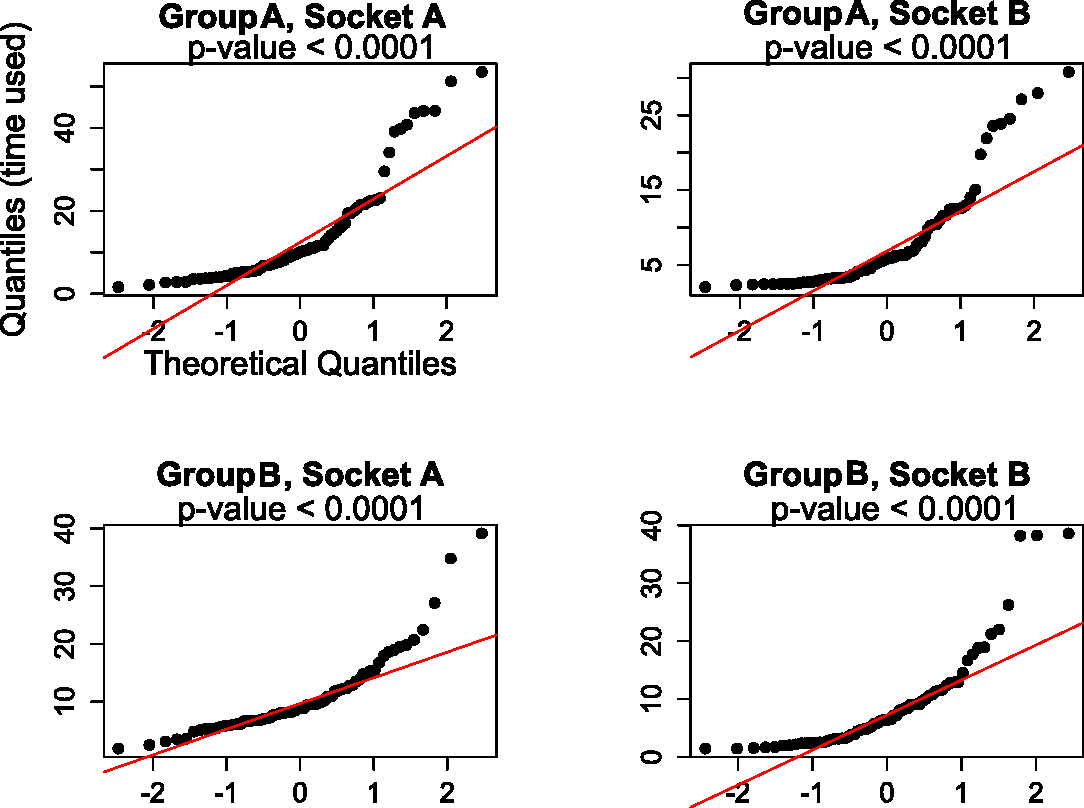
\includegraphics[width=0.9\textwidth]{./ch4-PiH/Figures/QQplot.pdf}
   \caption{Q-Q plots of time taken for four experiment conditions. The above p-values are from the Shapiro-Wilk test.}
   \label{QQplot}
\end{figure}


\begin{figure}
  \centering
  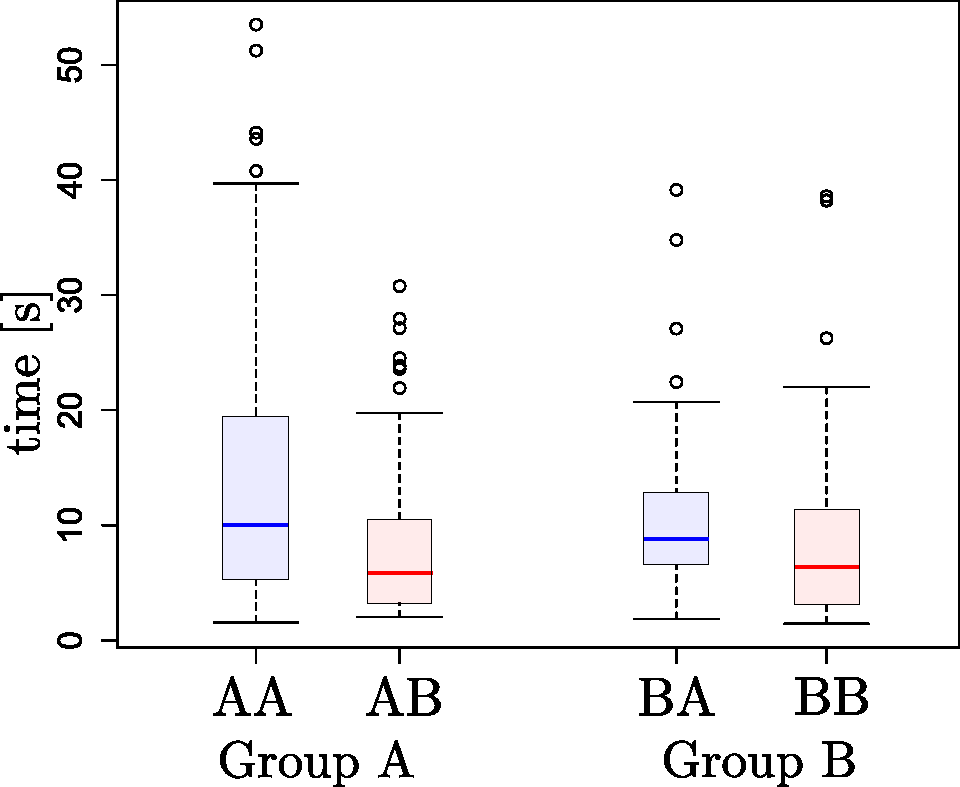
\includegraphics[width=0.8\textwidth]{./ch4-PiH/Figures/Group_Socket.pdf}
   \caption{Time taken to connect the sockets. For both groups, socket A always takes significantly longer time to connect, For Group A 
   p<0.0001 and for Group B p=0.0002.}
   \label{figuretimesubgroup}
\end{figure}

In summary, we observe that there is a significant effect of order. Starting with socket B greatly reduced the time 
taken for socket A (p=0.02). Regardless of the socket type between groups, the first socket always takes longer.
For AA vs BA, AA is significantly longer (p=0.02, Wilcoxon rank sum test). For socket B, BB vs AB, BB takes significantly
longer time (p<0.0001).


% 1) Is there are a difference across groups 
% 2) Is there a difference between the two sockets
%The null hypothesis is that there is no difference in the time taken to connect socket A or B. The result of the one-way anova
%is given in Table \ref{tab:ch4:anova_socket}. The null hypothesis is rejected at high significant level (***) indicating that 
%there is a difference between the sockets. According to the linear model it takes on average 4 seconds less to connect socket B 
%than it does for socket A.
%\begin{table}[h]
%\centering
%\begin{tabular}{lcc}
%  \hline
%          &   F    & Pr(>F)  	     \\ \hline
%   socket & 13.9   &  0.000232 *** 
%\end{tabular}
%\caption{One way anova of the time taken to connect two sockets A and B. There is a significant difference.}
%\label{tab:ch4:anova_socket}
%\end{table}
%We tested whether the group order had an effect on the connection time. We fitted a linear model
%with the predictor being time and the factors being the group (One or Two), the socket type (A or B) 
%and the subject's ID (1 to 10):
%\begin{equation}
% time = \beta_0 + \beta_1\, group + \beta_2\, socket + \beta_3\, subject
%\end{equation}
%and did the corresponding anova analysis on this linear model. We found that the difference between the sockets 
%remained significant.
\FloatBarrier
\section{EM policy search}\label{app:lb}
The objective of policy search in Reinforcement Learning (RL) is to optimise the parameters of a policy $\pi_{\Param}$
(which is a Gaussian Mixture Model (GMM) in our case) such to maximise a cost 
function, $J(\Param)$ Equation \ref{eq:ch4:app:J}, defined over the parameters of the policy:
%\begin{align}
%J(\Param)  &= \mathbb{E}_{\pi_{\Param}}\{R(\U,\B)\} \nonumber \\
%	   &= \sum\limits_{\B} d^{\pi}(\B) \sum\limits_{\U} \pi_{\Param}(\U,\B)\,R(\U,\B) \label{eq:ch4:app:J}
%\end{align}
%where $\B \sim d^{\pi}(\B)$ is the initial state distribution. The RL objective is to find a new set of parameters $\Param'$
%which maximises the above cost function $J$. Our approach follows the Monte-Carlo (MC) gradient estimate of Equation \ref{eq:ch4:app:J}
%through use of the log-likelihood ratio identity: $\nabla \log(\pi_{\Param}) = \nabla \pi_{\Param} / \pi_{\Param}$:


\begin{align}\label{eq:ch4:app:J}
 J(\Param) = \overbrace{\sum\limits_{i=1}^{N}   \underbrace{\left( \prod_{t=0}^{T^{[i]}} \pi_{\Param}(\U^{[i]}_t,\B^{[i]}_t) \right)}_{p_{\Param}(\tau_i)} \, R(\tau_i)}^{\mathbb{E}_{p_{\Param}}\{R\}} 
\end{align}

where $\tau_i = \{(\U_0,\B_0),\cdots,(\U_T^{[i]},\B_T^{[i]}) \}$ are the state-action samples of the $i$th episode. 
The total reward of one episode is the sum of discounted rewards:

\begin{equation}
 R(\tau_i) = \sum_{t=0}^{\mathrm{T^{[i]}}} \gamma^t \, r(\B^{[i]}_t,\U^{[i]}_t)
\end{equation}

where $\gamma \in [0,1)$ is the discount factor which dictates how much future rewards are considered important 
at the current decision point.
%\begin{align}
% \nabla_{\Param} J(\Param) &= \sum\limits_{\B} d^{\pi}(\B) \sum\limits_{\U}  \pi_{\Param}(\U,\B) \nabla_{\Param} \pi_{\Param}(\U,\B) \,R(\U,\B) \nonumber \\ 
%			   &= \mathbb{E}_{\pi_{\Param}}\{\nabla_{\Param} \log(\pi_{\Param}(\U,\B)) \,R(\U,\B)\} \label{eq:ch4:app:lJ}
%\end{align}
%This trick allows to evaluate the gradient of the parameters through Monte-Carlo trajectories generated from a the policy $\pi_{\Param}(\U,\B)$.
Most policy search methods are based gradient ascent on the cost function:
\begin{equation}
   \Param^{\mathrm{new}} =  \Param + \alpha\,\nabla_{\Param}J(\Param)
\end{equation}

The drawback of policy gradient methods is that a learning rate, $\alpha$, needs to be specified and the optimisation strongly depends 
on the fine tuning of this value. An alternative, which avoids
the learning rate problem, are Expectation-Maximisation (EM) methods. As our policy is a Gaussian Mixture Model (GMM) we can take advantage of 
the already existing EM updates of the GMM which are well known. Also updating the covariance parameters of the GMM by gradient ascent can lead 
to problems such the covariances being no longer positive-definite and this resolution requires the addition of constraints which becomes 
cumbersome. In contrast the EM solution for the GMM case is simple and easy to implement.

EM policy search methods have two phases. The first phase consists of generating a set of episodes $\boldsymbol{\tau}$ from 
the policy, this is the E-step. The second step consists of finding a new parameter $\Param^{\mathrm{new}}$ of the policy 
by maximising the cost function given the episodes:

\begin{equation}
  \Param^{\mathrm{new}} = \argmax\limits_{\Param} J(\Param) \label{eq:ch4:argmax}
\end{equation}

The above optimisation can be solved through the same approach taken in EM which consists of 
maximising the the logarithmic lower bound of the cost function $J(\Param)$: 

%The policy gradient theorem \cite{Sutton00policygradient} states the the gradient is:
%Steps taken to make a policy $\pi_{\Param}(\U,\B)$ maximise the objective function, .
%The policy will be maximised with respect to the lower bound of the cost function $J(\Param)$:
%\begin{align}
%  J(\Param') &= \sum_{i \in \mathbb{T}} \pi_{\Param'}(\Ui,\Bi)\, R(\Ui,\Bi) \nonumber\\ 
%	   &= \sum_{i \in \mathbb{T}}  \frac{\pi_{\Param'}(\Ui,\Bi)}{\pi_{\Param}(\Ui,\Bi)} \, \pi_{\Param}(\Ui,\Bi) \, R(\Ui,\Bi)
%\end{align}



\begin{align}
  \log( J(\Param) )  &= \log \sum\limits_{i=1}^{N} \frac{p_{\Param}(\tau_i)}{p_{\Param'}(\tau_i)} \, p_{\Param'}(\tau_i) \, R(\tau_i) \hspace*{2cm}  \nonumber \\
		     & \hspace*{2cm} \geq \underbrace{\sum\limits_{i=1}^{N} \log\Bigg( \frac{p_{\Param}(\tau_i)}{p_{\Param'}(\tau_i)}\Bigg) \, p_{\Param'}(\tau_i) \, R(\tau_i)}_{\mathcal{Q}(\Param,\Param')} \label{eq:lower_bound}
\end{align}
The parameter $\Param'$ belongs to the policy used to generate the episodes in the E-step and the parameter $\Param$ is the one 
we are optimising for. The lower bound $\mathcal{Q}(\Param,\Param')$ is derived from Jensen's inequality. 
The lower bound is next maximised by taking its derivative $\nabla_{\Param}\mathcal{Q}(\Param,\Param') = 0$. 
%We take the derivative of the lower bound of $\log(J(\Param'))$, Equation \ref{eq:lower_bound}, with respect to $\Param'$ and set it to 
%zero so as to maximise the cost function.

\begin{align}
 \nabla_{\Param}\mathcal{Q}(\Param,\Param')& = \sum\limits_{i=1}^{N} \nabla_{\Param} \log\big( p_{\Param}(\tau_i)\big) \, p_{\Param'}(\tau_i) \, R(\tau_i) - \hspace*{2cm} \nonumber \\
				    &\hspace*{2cm}\underbrace{\nabla_{\Param} \log\big( p_{\Param'}(\tau_i)\big)}_{=0} \, p_{\Param'}(\tau_i) \, R(\tau_i)				   
\end{align}
\begin{align}
 \nabla_{\Param}\mathcal{Q}(\Param,\Param') &= \mathbb{E}_{p_{\Param'}} \Big\{ \nabla_{\Param} \log\big( p_{\Param}(\tau_i)\big)\, R(\tau_i) \Big\} \label{eq:ch4:app:expec_Q}\\
					    &= \sum\limits_{i=1}^{N} \sum\limits_{t=0}^{T^{[i]}} \nabla_{\Param} \log\big( \pi_{\Param}(\Ui_t,\Bi_t)\big) \, R(\tau_i) \label{eq:ch4:app:logsum} \\
					    &= \sum\limits_{i=1}^{N} \sum\limits_{t=0}^{T^{[i]}} \nabla_{\Param}\log \pi_{\Param}(\U^{[i]}_t,\B^{[i]}_t) \, Q^{\pi_{\Param'}}(\U^{[i]}_t,\B^{[i]}_t) \label{eq:grad_log_cost_2}
\end{align}

From \ref{eq:ch4:app:expec_Q} to \ref{eq:ch4:app:logsum} we used the property: $\log( \prod \pi_{\Param} ) = \sum \log(\pi_{\Param})$ and 
the expectation vanishes as we evaluated it through sampling from the policy $\pi_{\Param'}$ (E-step). From \ref{eq:ch4:app:logsum} to \ref{eq:grad_log_cost_2} 
we used the fact that previous discounted rewards do not dependent on future time steps. The reader is referred 
to \cite[p. 50]{rl_gradient_survey_2013} for more details regarding Expectation-Maximisation and policy search in reinforcement learning.
In the next section \ref{app:grad} we maximise \ref{eq:grad_log_cost_2} for the case when the policy is parameterised by a GMM.


\section{Q-EM for GMM}\label{app:grad}

We derive the EM update rules of the lower bound $\mathcal{Q}(\Param,\Param')$ 
for a policy $\pi_{\Param}(\U,\B)$ parameterised by a Gaussian Mixture Model which we call 
Q-EM. Below we redefine the GMM function for convenience:

\begin{equation} \label{eq:ch5:app:gmm}
  \pi_{\Param}(\U,\B) = \sum\limits_{k=1}^K  \piK\,g(\U,\B;\MuK,\SigK)
\end{equation}

The parameters $\Param = \{w^{[k]},\MuK,\SigK\}_{1,\dots,K}$, are the weights, means and covariances 
of the individual Gaussian functions, $g(\cdot)$. 

Finding the new parameters of the GMM given a cost function $J(\Param)$ consists of maximising its logarithmic 
lower bound, Equation \ref{eq:ch4:app_div_Q}:

\begin{equation}\label{eq:ch4:app_div_Q}
  \nabla_{\Param}\mathcal{Q}(\Param,\Param') = \sum\limits_{i=1}^{N} \sum\limits_{t=0}^{T^{[i]}} \nabla_{\Param}\log \pi_{\Param}(\U^{[i]}_t,\B^{[i]}_t) \, Q^{\pi_{\Param'}}(\U^{[i]}_t,\B^{[i]}_t)
\end{equation}

As the ordering of the episode samples in the above equation does not mater we concatenate all the episodes into one dataset $\mathcal{D}$ 
and the $j$th sample in this dataset is given by $\mathbf{x}^{[j]} = [\U^{[j]},\B^{[j]}]^{\mathrm{T}}$. 

\begin{equation}\label{eq:ch4:app_div_Q_simple}
   \nabla_{\Param}\mathcal{Q}(\Param,\Param') = \sum\limits_{j=1}^{M} \nabla_{\Param}\log \pi_{\Param}(\mathbf{x}^{[j]}) \, Q^{\pi_{\Param'}}(\mathbf{x}^{[j]})
\end{equation}
To maximise Equation \ref{eq:ch4:app_div_Q_simple} we take the derivatives with respect to the 
parameters $\Param=\{w,\boldsymbol{\mu},\boldsymbol{\Sigma}\}$ of the GMM.  The reader my notice 
that the above equation is the derivative of the log-likelihood of the dataset $\mathcal{D}$ weighted
by $Q^{\pi_{\Param'}}$, a constant scalar value. As a consequence the result of maximisation will 
be similar to the standard EM solution of the GMM with an additional weighting factor. For a 
reference on the derivative of the log-likelihood of a GMM the reader is referred to \cite[p. 49]{matrix_ckb}
or \cite[Chap. 9]{Bishop_2006}.

%Setting the derivative of Equation \ref{eq:ch4:app_div_Q_simple} to zero and solving for the  
% we get a new weighted Maximisation update step in EM
%Making the substitution $\X = (\U,\B)^{\mathrm{T}}$ (small abuse of the notation) and  insuring a positive Q-function, $Q^{\pi}(\X^{[m]}) \geq 0$
%and by

\paragraph{Q-EM maximisation}

\begin{align}
    &\nabla_{\MuK} \mathcal{Q}(\MuK,\Param') =  \hspace*{5cm} \nonumber \\
    & \hspace*{1cm} \sum\limits_{j=1}^M \underbrace{\frac{\piK\,g(\Bx^{[j]};\MuK,\SigK)}{\sum\limits_{l=1}^{M} w^{[l]}\,g(\Bx;\Mu{l},\Sig{l}) } }_{\gamma_k(\Bx^{[j]})} \invSigK (\Bx^{[j]} - \MuK) \, \Qpx = 0 \label{eq:ch4:app:mu_max}
\end{align}

In \ref{eq:ch4:app:mu_max} we used the same notation and derivation as in \cite[Chap. 9.2.2]{Bishop_2006}, where $\gamma_k(\Bx^{[j]})$ is the responsibility factor, denoting 
the probability that data point $\mathbf{x}^{[j]}$ belongs to  Gaussian function $k$. After rearrangement the new mean is given by Equation \ref{eq:ch4:app_new_mu}.

\begin{empheq}[box={\tcbhighmath[colback=blue!2,colframe=blue]}]{align}
    \MuK_{\textrm{\textbf{new}}}    &= \frac{\sum\limits_{j=1}^{M} \gamma_k(\Bx^{[j]})\, \Qpx \, \Bx^{[j]} }{\sum\limits_{j=1}^{M} \gamma_k(\Bx^{[j]})\, \Qpx} \label{eq:ch4:app_new_mu} \\
    & \nonumber\\
    \SigK_{\textrm{\textbf{new}}}   &= \frac{\sum\limits_{j=1}^{M}  \gamma_k(\Bx^{[j]})\, \Qpx (\Bx^{[j]} - \MuK)(\Bx^{[j]} - \MuK)^{\mathrm{T}} }{ \sum\limits_{j=1}^{M} \gamma_k(\Bx^{[j]})\, \Qpx } \label{eq:ch4:app_new_cov}  \\
    & \nonumber\\
    w^{[k]}_{\textrm{\textbf{new}}} &= \frac{\sum\limits_{j=1}^{M} \Qpx \, \gamma_k(\Bx^{[j]})}{\sum\limits_{j=1}^{M} \Qpx} \label{eq:ch4:app_new_pi}
\end{empheq}

The covariances, Equation \ref{eq:ch4:app_new_cov}, and weights, Equation \ref{eq:ch4:app_new_pi}, are derived in a similar fashion.

%\begin{align}
%\nabla_{\Muk} \log J(\Param) =& \sum\limits_{m=1}^{M} \alpha(z_{mk})\, Q(\Xm)\, \invSigK (\Xm - \MuK) = 0 \nonumber \\
%			 \MuK_{\textrm{\textbf{new}}} =& \frac{\sum\limits_{m=1}^{M} \alpha(z_{mk})\, Q(\Xm)\, \Xm }{\sum\limits_{j=1}^{M} \alpha(z_{jk})\, Q(\X^{[j]})}
%\end{align}
%\begin{equation}
% \alpha(z_{mk}) = \frac{w^{[k]} \cdot g(\Xm;\MuK,\SigK)}{\sum\limits_{j=1}^{K}w^{[j]} \cdot g(\Xm;\boldsymbol{\mu}^{[j]},\boldsymbol{\Sigma}^{[j]})}
%\end{equation}

%\subsection{M-step}\label{app:Q-EM}
%Given a set of points $\X = (\U,\B)^{\mathrm{T}}$ and  a positive Q-function, $Q^{\pi}(\X^{[m]}) \geq 0$
%and by setting the derivative of Equation \ref{eq:grad_log_cost} to zero and solving for the parameters
%$\Param=\{w,\boldsymbol{\mu},\boldsymbol{\Sigma}\}$ we get a new weighted Maximisation updates in EM:
%\begin{align}
% w^{[k]}_{\textrm{\textbf{new}}} &= \frac{\sum\limits_{m=1}^{M} Q^{\pi}(\X^{[m]})\, \alpha(z_{mk})}{\sum\limits_{j=1}^{M} Q^{\pi}(\X^{[j]})} \\
% \MuK_{\textrm{\textbf{new}}}     &= \frac{\sum\limits_{m=1}^{M} \alpha(z_{mk})\, Q^{\pi}(\Xm)\, \Xm }{\sum\limits_{j=1}^{M} \alpha(z_{jk})\, Q^{\pi}(\X^{[j]})} \\
% \SigK_{\textrm{\textbf{new}}}    &= \frac{\sum\limits_{m=1}^{M} Q^{\pi}(\Xm)\, \alpha(z_{mk})\, (\Xm - \MuK)(\Xm - \MuK)^{\mathrm{T}} }{ \sum\limits_{j=1}^{M} Q^{\pi}(\X^{[j]})\, \alpha(z_{jk}) }
%\end{align}
%$\alpha(z_{mk})$ is the responsibility factor, denoting the probability that data point $m$ is a member of the 
%Gaussian function $k$ (see \cite[Chap. 9]{Bishop_2006}).

\section{Unbiased estimator}\label{app:unbiased_delta}

%\begin{equation}
%  \delta^{\pi}_t = r_{t+1} + \gamma V^{\pi}(b_{t+1}) - V^{\pi}(b_t) \\
%\end{equation}
The temporal difference error is an unbiased estimate of the advantage function:
\begin{align}
  \displaystyle \mathop \mathbb{E}_{\pi_{\Param}} \{ \delta^{\pi}_t|b_t,u_t\} &=  \mathop\mathbb{E}_{\pi_{\Param}}\{ r_{t+1} + \gamma V^{\pi}(b_{t+1})|b_t,u_t\} - V^{\pi}(b_t) \nonumber \\
									   &= Q^{\pi}(b_t,u_t) - V^{\pi}(b_t) \nonumber \\
									   &= A^{\pi}(b_t,u_t)
\end{align}


\chapter{Non-parametric Bayesian State Space Estimator}\label{ch5:appendix}

%\subsection{EKF-SLAM models}
%\paragraph{Motion update}
%\begin{align}
%  \bar{\mu}_t      &= f(\mu_{t-1},u_t)\\
%  \bar{\Sigma}_{t} &= F \Sigma_{t-1} F^{\mathrm{T}} + Q
%\end{align}
%Where $F = \left[\frac{\partial f(\mu_{t-1},u_t)}{\partial \mu_{t-1} } \right]$ is the Jacobian of the dynamic model with respect to the Gaussian mean. The 
%bar notation on the mean and covariance is to indicate that no sensing information has been used to update their estimates.
%\paragraph{Measurement update}
%\begin{align}
%   K    &= \bar{\Sigma}_{t} H (H \bar{\Sigma}_{t} H + R)^{-1} \\
%  \mu_t &= \bar{\mu}_t + K \cdot (Y_t - \hat{Y}_t)\\
%  \Sigma_t &= (I - KH) \bar{\Sigma}_{t}
%\end{align}
%Where $H = \left[\frac{\partial h(\mu_A,\mu_O;\beta)}{\partial \mu_A\mu_O}\right]$ is the Jacobian of the measurement function (Equation \ref{eq:ekf-measurement_function})  
%with respect to the mean of the joint distribution. 

%\subsection{Bayesian joint to filter}\label{appendix:bayes_joint}
%\begin{align}
%&P(A_t,O,Y_{0:t},u_{1:t})\\
%&= P(O) \left( \sum_{A_{0:t-1}}  P(A_0) \prod_{t=0}^{t} P(A_t|A_{t-1},u_{t}) P(Y_t|A_t,O) \right)  P(Y_t|A_t,O) \\
%&= P(O) \left( \sum_{A_{0:t-1}} P(A_{0:t},Y_{0:t-1},u_{1:t}) \right)  \\
%&= P(O) P(A_t,Y_{0:t},u_{1:t}) \\
%&= P(A_t,O,Y_{0:t},u_{1:t})
%\end{align}

\section{Probabilities}

There are two rules extensively used in the derivation of a Bayesian filter recursion regardless 
of the chosen parameterisation. Although well known we restate them here for convenience.

\begin{itemize}
 \item \textbf{Chain rule}\\
 \begin{equation}
  P(X_M,\cdots,X_1) = P(X_M|X_{M-1},\cdots,X_1) P(X_{M-1},\cdots,X_1) \label{eq:ch5:chain_rule}
 \end{equation}
 \item \textbf{Conditional independence}\\
  \begin{align}
    P(A,B|C) &= P(A|\Ccancel[red]{B},C) P(B|C) \nonumber \\
             &= P(A|C) P(B|C)
  \end{align}
  $A$ and $B$ are independent given that $C$ is known.
\end{itemize}


\section{Bayesian filtering recursion}\label{appendix:bayes_recursion}

\paragraph{Joint distribution}\\

The joint distribution is over all the random variables since $t=0$ until the current 
time step $t$:
\begin{align}
 &P(A_{0:t},O,Y_{0:t}|u_{1:t}) =\nonumber \\ 
 &P(A_0)P(O)P(Y_0|A_0,O)\prod_{t=1}^t P(A_t|A_{t-1},u_{t}) P(Y_t|A_t,O) \label{eq:ch5:app:joint} \\
 &P(A_0)P(O)P(Y_0|A_0,O) P(A_{1:t}|u_{1:t}) P(Y_{1:t}|A_{1:t},O)  \label{eq:ch5:app:joint_2} \\
 &P(A_0)P(O) P(A_{1:t}|u_{1:t}) P(Y_{0:t}|A_{0:t},O) \label{eq:ch5:joint_final}
\end{align}

From Equation \ref{eq:ch5:app:joint} to \ref{eq:ch5:app:joint_2} we made use of the chain rule 
of probabilities (Equation \ref{eq:ch5:chain_rule}) and the conditional independence $A_{t+1} \independent A_{t-1} | A_t$, see below a more concrete example for $P(A_{0:3}|u_{1:3})$:
\begin{align}
  &P(A_3,A_2,A_1,A_0|u_{1:3}) = \nonumber \\ 
  &P(A_3|A_2,\Ccancel[red]{A_1},\Ccancel[red]{A_0},u_{1:3})P(A_2|A_1,\Ccancel[red]{A_0},u_{1:3})P(A_1|A_0,u_{1:3}) P(A_0|u_{1:3}) = \label{eq:ch5:chain_example} \\
  &P(A_3|A_2,u_3,\Ccancel[red]{u_{1:2}})P(A_2|A_1,u_2,\Ccancel[red]{u_{1,3}})P(A_1|A_0,u_1,\Ccancel[red]{u_{2:3}}) P(A_0|\Ccancel[red]{u_{1:3}}) = \label{eq:ch5:cancel_actions} \\
  &\underbrace{(A_3|A_2,u_3) P(A_2|A_1,u_2) P(A_1|A_0,u_1)}_{P(A_{1:3}|u_{1:3})} P(A_0)
\end{align}

We applied the chain rule to get Equation \ref{eq:ch5:chain_example} and the cancellations arise from 
conditional independence between the agent random variable $A_t$ specified by the BN, 
see Figure \ref{fig:bayesian_sse_dag} on page \pageref{fig:bayesian_sse_dag}. The cancellations on line \ref{eq:ch5:cancel_actions}
arise also from BN, $A_t$ only depends on $u_t$ and no previous actions.


To see clearer the relationship between the left and right hand side of Equation \ref{eq:ch5:joint_final}, 
we can again apply the chain rule to the right, which gives:
\begin{align}
 P(A_{0:t},O,Y_{0:t}|u_{1:t}) &=  P(Y_{0:t}|A_{0:t},O,\Ccancel[red]{u_{1:t}}) P(A_{0:t},O|u_{1:t}) \\
			      &=  P(Y_{0:t}|A_{0:t},O) P(A_{0:t},O|u_{1:t})
\end{align}
The measurements $Y_{0:t}$ are independent of the actions $u_{0:t}$  given the history of the agent's random 
variables $A_{0:t}$. Next we see the relation between the thirst three terms on the right of Equation \ref{eq:ch5:joint_final}
with $P(A_{0:t},O|u_{1:t})$. We apply the chain rule:

\begin{align}
 P(A_{0:t},O|u_{1:t}) &= P(A_{0:t}|\Ccancel[red]{O},u_{1:t}) P(O|\Ccancel[red]{u_{1:t}}) \\
		      &= P(A_0) P(O) P(A_{1:t}|u_{1:t}) 
\end{align}

The object $O$ is conditionally independent of the actions and the second of actions $A_{0:t}$ are conditional independent 
of the object as they are dependent only on the measurements.

Typically we are interested in the filtered joint distribution $P(A_t,O,Y_{0:t}|u_{1:t})$ which 
is obtained by marginalising over $A_{0:t-1}$:
\begin{equation}
  P(A_t,O,Y_{0:t}|u_{1:t}) = \sum_{A_{0:t-1}}  P(A_t,A_{0:t-1},O,Y_{0:t}|u_{1:t}) \\
\end{equation}
A recursion exists making it not necessary to sum over all agents random variables from the state time 
until then end, but instead we only have to consider the last time step, see the next paragraph.

%  P(A_{0:t},O,Y_{0:t},u_{1:t})  &= P(A_0)P(O)\prod_{t=1}^{t} P(A_t|A_{t-1},u_{t-1}) P(Y_t|A_t,O) \\
\paragraph{Filtering problem}\\
We derive $P(A_t,O,Y_{0:t}|u_{1:t})$, we start from the joint distribution, Equation \ref{eq:br_chain}:
\begin{equation}
   P(A_t,O,Y_{0:t}|u_{1:t})  = \sum_{A_{t-1}} P(A_t,A_{t-1},O,Y_t,Y_{0:t-1}|u_{t},u_{1:t-1}) \label{eq:br_chain} 
\end{equation}

\begin{tabular}{lll}
   $P(A_t,O,Y_{0:t}|u_{1:t})$ & $=\sum_{A_{t-1}}$ &  $P(Y_t|\Ccancel[red]{Y_{0:t-1}},A_t,\cancel{A_{t-1}},O,\cancel{u_{t}},\cancel{u_{1:t-1}}) $ \\
			      &  & $P(A_t|A_{t-1},\Ccancel[red]{O},u_{t},\Ccancel[red]{Y_{0:t-1}},\Ccancel[red]{u_{1:t-1}}) $ \\
			      &  & $P( A_{t-1},O,Y_{0:t-1}|\Ccancel[red]{u_t},u_{1:t-1})$
\end{tabular}

\begin{align}
  &P(A_t,O,Y_{0:t}|u_{1:t}) \\
  &= \sum_{A_{t-1}} P(Y_t|A_{t},O)  P(A_t|A_{t-1},u_{t})  P(A_{t-1},O,Y_{0:t-1}|u_{1:t-1}) \nonumber \\
  &= P(Y_t|A_{t},O)  \underbrace{\sum_{A_{t-1}} P(A_t|A_{t-1},u_t)  P(A_{t-1},O,Y_{0:t-1}|u_{1:t-1})}_{P(A_t,O,Y_{0:t-1}|u_{1:t})} 
\end{align}

\begin{align}
   P(A_t,O,Y_{0:t}|u_{1:t}) &= P(Y_t|A_{t},O)  P(A_t,O,Y_{0:t-1}|u_{1:t}) \nonumber \\
			    &= P(Y_t|A_{t},O)  P(A_t,O|Y_{0:t-1},u_{1:t})  P(Y_{0:t-1}|u_{1:t})
\end{align}

All the cancellations come from the \textit{Markov Assumption} read from the structure of the Bayesian network.
The resulting final Bayesian recursion is obtained by conditioning on the measurement and actions, which is the normalisation factor.

\begin{align}\label{eq:ch5_measurement_update}
 P(A_t,O|Y_{0:t},u_{1:t}) &= \frac{P(Y_t|A_{t},O)  P(A_t,O|Y_{0:t-1},u_{1:t})  P(Y_{0:t-1}|u_{1:t})}{P(Y_{0:t}|u_{1:t})} \nonumber \\
			  &= \frac{P(Y_t|A_{t},O)  P(A_t,O|Y_{0:t-1},u_{1:t})  \Ccancel[red]{P(Y_{0:t-1},u_{1:t})}}{P(Y_t|Y_{0:t-1},u_{1:t}) \Ccancel[red]{P(Y_{0:t-1}|u_{1:t})}}   
\end{align}
 
\begin{equation}
   P(A_t,O|Y_{0:t},u_{1:t}) = \frac{P(Y_t|A_{t},O) P(A_{t},O|Y_{0:t-1},u_{1:t})}{P(Y_t|Y_{0:t-1},u_{1:t})} \label{eq:ch5:app:bayes_filter}
\end{equation}

The evidence is the the integration of all terms which are not measurements in the numerator of Equation \ref{eq:ch5:app:bayes_filter}.

\begin{align}
 P(Y_t|Y_{0:t-1},u_{1:t}) &= \sum\limits_{A_t} \sum\limits_O  P(Y_t|A_{t},O) P(A_{t},O|Y_{0:t-1},u_{1:t}) \\
			  &= \sum\limits_{A_t} \sum\limits_O  P(Y_t,A_{t},O|Y_{0:t-1},u_{1:t})
\end{align}
This is very expensive since we have to sum over the entire joint distribution, the MLMF avoids doing this by only considering the dependent 
regions of the joint distribution.

\section{Recursion example}\label{appendix:recursion_example}

Derivation of the filtered joint distribution, $P(A_t,O,Y_t|Y_{0:t},u_{1:t})$, for 
two updates. At initialisation when no action has yet been taken the filtered joint distribution 
is the product of the initial marginals and first likelihood function:
\begin{equation}
  P(A_0,O,Y_0) = P(O) P(A_0) P(Y_0|A_0,O) 
\end{equation}
  
The a first action, $u_1$ is applied, which to get the filtered joint distribution is marginalised:
\begin{align}
  P(A_1,O,Y_0|u_1) &= P(O)\sum\limits_{A_0} P(A_1|A_0,u_1) P(A_0) P(Y_0|A_0,O)\\
                   &= P(O)\sum\limits_{A_0} P(A_1,A_0,Y_0|u_1,O)\\
                   &= P(O) P(A_1,Y_0|u_1,O) \label{eq:ch5:rec_ex1}\\
                   &= P(O) P(Y_0|A_1,O,u_1) P(A_1|u_1,\Ccancel[red]{O}) \label{eq:ch5:rec_ex2}\\
                   &= P(O) P(Y_0|A_1,O,u_1) P(A_1|u_1) 
\end{align} 
From Equation \ref{eq:ch5:rec_ex1} to \ref{eq:ch5:rec_ex2} we used the Chain rule \ref{eq:ch5:chain_rule} and 
the cancellation in Equation \ref{eq:ch5:rec_ex2} arise from the factorisation of the joint distribution, 
see Figure \ref{fig:bayesian_sse_dag} on page \pageref{fig:bayesian_sse_dag}, $A$'s marginal does not depend on $O$.
After the application of the first action, the filtered joint has the following form:
\begin{equation}
 P(A_1,O,Y_0|u_1) = P(O) P(A_1|u_1) P(Y_0|A_1,O,u_1)
\end{equation}
A second measurement $Y_1$ and action $u_2$ are integrated into the filtered joint distribution:
\begin{align}
 &P(A_2,O,Y_{0:1}|u_{1:2}) = \nonumber \\
 &P(O) \sum\limits_{A_1} P(A_2|A_1,u_2) P(A_1|u_1) P(Y_0|A_1,O,u_1) P(Y_1|A_1,O) = \nonumber\\
 &P(O) \sum\limits_{A_1} P(A_2,A_1|u_{1:2}) P(Y_{0:1}|A_1,O,u_1) = \nonumber \\
 &P(O) \sum\limits_{A_1} P(A_2,A_1,Y_{0:1}|O,u_{1:2}) = \nonumber \\
 &P(O) P(A_2,Y_{0:1}|O,u_{1:2}) = \\
 &P(O) P(Y_{0:1}|A_2,O,u_{1:2})P(A_2|\Ccancel[red]{O},u_{1:2}) \label{eq:ch5:rec_ex3} 
\end{align}
We expand the function $P(Y_{0:1}|A_2,O,u_{1:2})$ to give a sense of how the likelihood function's positions 
get as illustrated in Figure \ref{fig:discrete_example} on page \pageref{fig:discrete_example}.

\begin{align}
  P(Y_0,Y_1|A_2,O,u_1,u_2) &= P(Y_0|\Ccancel[red]{Y_1},A_2,O,u_1,u_2) P(Y_1|A_2,O,\Ccancel[red]{u_1},u_2) \\
		           &= P(Y_0|A_2,O,u_{1:2}) P(Y_1|A_2,O,u_2)
\end{align}
The first likelihood of measurement $Y_0$ is dependent on the last to applied actions whilst the likelihood
of $Y_1$ is dependent on the last action.
 
 %&P(O) P(A_2|u_{1:2}) P(Y_0|A_2,O) P(Y_1|A_2,O) \label{eq:ch5:rec_ex4}
 %\end{align}
%From Equation \ref{eq:ch5:rec_ex3} to \ref{eq:ch5:rec_ex4} we did the same steps as for Equation \ref{eq:ch5:rec_ex1} to \ref{eq:ch5:rec_ex2}.
Repeating the above for $Y_{2:t}$ and $u_{3:t}$ results in:
\begin{equation}
 P(A_t,O,Y_{0:t}|u_{1:t}) = P(O)P(A_t|u_{1:t}) \prod_{i=0}^{t} P(Y_i|A_t,O,u_{i+1:t})
\end{equation}
If $t=3$, ($Y_{0:3}$ and $u_{1:3}$) according to the above equation we would get:
\begin{align}
 P(A_3,O,Y_{0:3}|u_{1:3}) = P(O)P(A_3|u_{1:3}) &P(Y_0|A_3,O,u_{1:3}) \nonumber \\
					       &P(Y_1|A_3,O,u_{2:3}) \nonumber \\
					       &P(Y_2|A_3,O,u_{3:3}) \nonumber \\
					       &P(Y_3|A_3,O,\Ccancel[red]{u_{4:3}})
\end{align}
We introduce some notation rules, first if $(i+1) > t$ for $u_{(i+1):t}$ then it cancels out since the current
measurement $Y_t$ cannot depend on a future action $u_{(i+1)}$.

\section{Derivation of the evidence}\label{appendix:evidence}

%From first principle, Equation \ref{eq:marginal_likelihood_memory}, we demonstrated that 
%the marginal likelihood (also called evidence) is simply the difference
%in the probability mass located inside the measurement functions after applying $P(Y_t|A_t,O)$.

The evidence, also known as the marginal likelihood, is the marginalisation of all non measurement random variables from 
the filtered joint distribution $P(A_t,O,Y_{0:t}|u_{1:t})$. We detail below how we compute the evidence in a recursive 
manner whilst only considering dependent regions of the joint distribution.

We start with the \textbf{standard} definition of the evidence:
\begin{equation}\label{eq:ch5:numerator}
 P(Y_{0:t}|u_{1:t}) = \sum\limits_{A_t}\sum\limits_{O} P(A_t,O,Y_{0:t}|u_{1:t}) \in \mathbb{R}
\end{equation}
If both $A_t$ and $O$ are random variables defined over a discretised state space of $N$ states,
the above double integral will sum a total of $N^2$ states which is the complete state space of the 
joint distribution $P(A_t,O,Y_{0:t}|u_{1:t}) \propto  P(A_t,O|Y_{0:t},u_{1:t})$, see Figure \ref{fig:maringal_joint_example_v2} 
on page \pageref{fig:maringal_joint_example_v2} for an illustrate of such a joint distribution.
As we are interested in a recursive computation of the evidence, we consider the gradient:
\begin{align}
  \alpha_t = \nabla_{Y_t}P(Y_{0:t}|u_{1:t}) =  P(Y_{0:t}|u_{1:t}) - P(Y_{0:t-1}|u_{1:t})
\end{align}

\begin{align}
 \alpha_t  &= \sum\limits_{A_t}\sum\limits_{O} P(A_t,O,Y_{0:t}|u_{1:t}) - P(A_t,O,Y_{0:t-1}|u_{1:t})  \\
	   &= \sum\limits_{A_t}\sum\limits_{O} P(Y_t|A_t,O)P(A_t,O,Y_{0:t-1}|u_{1:t}) - P(A_t,O,Y_{0:t-1}|u_{1:t}) \\
	   &= \sum\limits_{A_t}\sum\limits_{O} (P(Y_t|A_t,O) - 1)P(A_t,O,Y_{0:t-1}|u_{1:t}) \label{eq:ch5:gradient_alpha}
\end{align}
The gradient $\alpha_t$ is the difference in mass before and after the application the likelihood function, $P(Y_t|A_t,O)$. The above 
summation, Equation \ref{eq:ch5:gradient_alpha}, is over the entire joint distribution state space. We can take advantage of the fact 
that the likelihood function is sparse and will only affect a small region of the joint distribution, which we called the dependent states, $\cap$.
The states which are not affected by the joint distribution will result in a contribution of zero to Equation \ref{eq:ch5:gradient_alpha}. We 
rewrite the gradient update in terms of only the dependent regions:

\begin{equation}
 \alpha_t = \sum\limits_{A_t}\sum\limits_{O} (P(Y_t|A_t,O) - 1)P_{\cap}(A_t,O,Y_{0:t-1}|u_{1:t})
\end{equation}

Consider the first update of the evidence at time $t=0$:

\begin{align}
 \alpha_0 &= \sum\limits_{A_t}\sum\limits_{O} (P(Y_0|A_0,O) - 1)P(A_0,O) 
\end{align}
The one in Equation \ref{eq:ch5:evidence_yo} is the original value of the normalisation denominator before any observation is made and as the 
initial joint distribution $P(A_0,O)$ is normalised the value of the denominator is one.
\begin{equation}
 P(Y_0) = 1 + \alpha_0 \label{eq:ch5:evidence_yo}
\end{equation}
For the evidence $P(Y_{0:t}|u_{1:t})$ we consider the summation of all the derivatives $\alpha_t$ from time $t=0$ until $t$:
\begin{equation}
 P(Y_{0:t}|u_{1:t}) = 1 + \sum_{t=0}^t \alpha_t \label{eq:ch5:evidence_y}
\end{equation}


%\begin{align}
% \alpha_0 &= \sum\limits_{A_t}\sum\limits_{O} P(A_0,O) - \sum\limits_{A_t}\sum\limits_{O} P(Y_0|A_0,O) \cdot P(A_0,O) \\
%        &= \sum\limits_{A_t}\sum\limits_{O} P(A_0,O) - P(Y_0|A_0,O) \cdot P(A_0,O) \\
%        &= \sum\limits_{A_t}\sum\limits_{O} P(A_0,O) - P(A_0,O,Y_0)
%\end{align}

%\begin{align}
% P(Y_0) = \sum\limits_{A_t} \sum\limits_O P(A_0,O) = 1\\
% \sum\limits_{A_t} \sum\limits_O P(A_t,O|Y_{0:t-1}) = 1
%\end{align}

 %\begin{align}
 % \sum\limits_{A_t}\sum\limits_{O} P(Y_0|A_0,O) \cdot P(A_0,O)  &\overbrace{\leq \sum\limits_{A_t}\sum\limits_{O} P(A_0,O)}^{=1} \label{eq:ch5:less1_1}\\
 % \sum\limits_{A_t}\sum\limits_{O} P(Y_0|A_0,O) \cdot P(A_0,O) &\leq 1 \label{eq:ch5:less1_2} \\
 % P(Y_0) &\leq 1 \\
 %  P(Y_0) &= 1 - \alpha_0 \label{eq:marginal_likelihood_equal_I}
%\end{align}

%\begin{align}
%\alpha_0 &= \sum\limits_{A_t}\sum\limits_{O} P(A_0,O) - \sum\limits_{A_t}\sum\limits_{O} P(Y_0|A_0,O) \cdot P(A_0,O) \\
%       &= \sum\limits_{A_t}\sum\limits_{O} P(A_0,O) - P(Y_0|A_0,O) \cdot P(A_0,O) \\
%        &= \sum\limits_{A_t}\sum\limits_{O} P(A_0,O) - P(A_0,O,Y_0)
%\end{align}



 
%\begin{align}
%   P(Y_{0:t})         &= P(Y_t|Y_{0:t-1}) P(Y_{0:{ t-1}})\\
%   P(Y_{t}|Y_{0:t-1}) &= \sum\limits_{A_t} \sum\limits_O P(A_t,O,Y_t|Y_{0:t-1}) \\
%              &= \sum\limits_{A_t} \sum\limits_O P(Y_t|A_t,O) P(A_t,O|Y_{0:t-1}) 
%\end{align}

 
 
 %\begin{align}
 % I\_tmp &= \sum\limits_{A_t}\sum\limits_{O} (1 - P(Y_t|A_t,O)) P(A_t,O,Y_{0:t-1})\\
 %        &= \sum\limits_{A_t}\sum\limits_{O} P(A_t,O,Y_{0:t-1}) - P(Y_t|A_t,O)P(A_t,O,Y_{0:t-1})\\
 %        &= \sum\limits_{A_t}\sum\limits_{O} P(A_t,O,Y_{0:t-1}) - P(A_t,O,Y_{0:t})\\
 % Is     &= Is + I\_tmp \\
 % PYs   &= 1 - Is
 %\end{align}

 
 
%\begin{align}
% &P(Y_{0:t}) = \sum\limits_{A_t}\sum\limits_{O} P(Y_t|A_t,O)\cdot P(A_t,O,Y_{0:t-1}) 
%		  &= \sum\limits_{A_t}\sum\limits_{O} P(Y_t|A_t,O)\cdot \Big(P_{\ominus}(A_t,O,{\color{red}Y_{0:t-1}}|u_{1:t}) + P_{\cap}(A_t,O,Y_{0:t-1}|u_{1:t})\Big)\\
%		  &= \sum\limits_{A_t}\sum\limits_{O} P_{\ominus}(A_t,O,{\color{red}Y_{0:t}}|u_{1:t}) + P(Y_t|A_t,O)\cdot P_{\cap}(A_t,O,Y_{0:t-1}|u_{1:t}) \label{eq:marginal_likelihood_memory_last}
%\end{align}

%In Equation \ref{eq:ch5:less1_1}, we use the fact that after applying the measurement likelihood function, which lies in the interval $0 \leq P(Y_t|A_t,O) \leq 1$, 
%to the joint distribution, its sum will always be smaller or equal to $1$.
%From Equation \ref{eq:ch5:less1_1} to \ref{eq:ch5:less1_2} we use the fact that $P(A_t,O|Y_{0:t-1})$ is a probability density and must sum to 1.

%\begin{align}
%  \sum\limits_{A_t}\sum\limits_{O} P(Y_t|A_t,O) \cdot P(A_t,O|Y_{0:t-1})  &\overbrace{\leq \sum\limits_{A_t}\sum\limits_{O} P(A_t,O|Y_{0:t-1})}^{=1} \label{eq:ch5:less1_1}\\
%  \sum\limits_{A_t}\sum\limits_{O} P(Y_t|A_t,O) \cdot P(A_t,O|Y_{0:t-1}) &\leq 1 \label{eq:ch5:less1_2} \\
%  P(Y_t|Y_{0:t-1}) &\leq 1 \\
%  P(Y_t|Y_{0:t-1}) + \alpha &= 1 \label{eq:marginal_likelihood_equal_I}
%\end{align}
%We equate Equation \ref{eq:marginal_likelihood_equal_I} with \ref{eq:marginal_likelihood_memory_last} and find a solution for the marginal likelihood which
%only depends on areas of the joint distribution which are dependent.
		   
%\begin{align}		  
% &\overbrace{\sum\limits_{A_t}\sum\limits_{O} P(A_t,O|Y_{0:t-1})}^{=1} - \alpha  = \sum\limits_{A_t}\sum\limits_{O} P(A_t,O,Y_{0:t}) + P(Y_t|A_t,O)P(A_t,O,Y_{0:t-1})
%\end{align}

%\begin{align}   
%   \alpha &= \sum\limits_{A_t}\sum\limits_{O}  \overbrace{P_{\ominus}(A_t,O|Y_{0:t-1}) + P_{\cap}(A_t,O|Y_{0:t-1})}^{P(A_t,O|Y_{0:t-1})}\nonumber\\ %
%	  & - P_{\ominus}(A_t,O,Y_{0:t}) - P(Y_t|A_t,O)\cdot P_{\cap}(A_t,O,Y_{0:t-1}) \\
%    \alpha &= \sum\limits_{A_t}\sum\limits_{O} P_{\cap}(A_t,O|Y_{0:t-1}) - P(Y_t|A_t,O)\cdot P_{\cap}(A_t,O|Y_{0:t-1}) \\
%	   &= \sum\limits_{A_t}\sum\limits_{O} P_{\cap}(A_t,O|Y_{0:t-1}) (1 - P(Y_t|A_t,O)) \label{eq:marginal_likelihood_equal_I2}
%\end{align}

%The last line, Equation \ref{eq:marginal_likelihood_equal_I2}, when substituted back into line \ref{eq:marginal_likelihood_equal_I}, tells us that the 
%normalisation factor or marginal likelihood is $1$ minus the difference in the area of dependence a priori to the application of 
%the measurement function, Equation \ref{eq:marginal_liklihood_final}.

%\begin{equation}\label{eq:marginal_liklihood_final}
% P(Y_t|Y_{0:t}) = 1 - \alpha
%\end{equation}


\section{Derivation of the marginal}\label{appendix:marginal}

The marginal of a random variable is the marginalisation or integration over all other random variables, $P(A_t,|Y_{0:t}) = \sum\limits_{O} P(A_t,O|Y_{0:t})$. Below 
we give a form of this integration which exploits the independent regions in the joint distribution.

\begin{equation} \label{eq:ch5:app:dummy}
 P(A_t,|Y_{0:t}) = \mathbf{P(A_t|Y_{0:t-1})} - \Big(\mathbf{P(A_t|Y_{0:t-1})} - P(A_t|Y_{0:t}) \Big) 
\end{equation}

In Equation \ref{eq:ch5:app:dummy} we add and substract $P(A_t|Y_{0:t-1})$ and we further split 
$P(A_t|Y_{0:t-1})$ into independent and dependent components: 

\begin{align}
  &P(A_t,|Y_{0:t}) =  P(A_t|Y_{0:t-1}) - \nonumber \\ 
  &\Big(\underbrace{P_{\cap}(A_t|Y_{0:t-1}) + \Ccancel[red]{P_{\ominus}(A_t|Y_{0:t-1})}}_{P(A_t|Y_{0:t-1})} -  \underbrace{P_{\cap}(A_t|Y_{0:t}) + \Ccancel[red]{P_{\ominus}(A_t|Y_{0:t})}}_{P(A_t|Y_{0:t})})   \Big) \label{eq:dependence1} 
\end{align}
From equation \ref{eq:dependence1} to \ref{eq:dependence2} we used the fact that independent regions of the marginal distributions will remain unchanged after
an observation, $P_{\ominus}(A_t|Y_{0:t-1}) = P_{\ominus}(A_t|Y_{0:t})$, and before re-normalisation. This results in the final recursive update:
\begin{equation}
 P(A_t,|Y_{0:\color{red}{t}}) =  P(A_t|Y_{0:\color{red}{t-1}}) - \Big(P_{\cap}(A_t|Y_{0:t-1}) -  P_{\cap}(A_t|Y_{0:t})  \Big) \label{eq:dependence2} 
\end{equation}
Equation \ref{eq:dependence2} states that only elements of the marginals which are dependent will change by the difference
before and after a measurement update.

 
\end{appendices}

